En este capítulo se presentan los detalles de diseño del proyecto, basándonos en
el análisis mostrado en los anteriores apartados. Se detallan la arquitectura
general y el diseño físico de datos entre otros aspectos.

\section{Arquitectura del sistema}

\subsection{Arquitectura física}
\label{sec:arquitectura-fisica}

En este apartado, describimos los principales componentes hardware que forman la
arquitectura física de nuestro sistema, recogiendo por un lado los componentes
del servidor de producción y, por otro lado, los componentes del cliente de acceso.

\subsubsection{Servidor de producción}
\label{subsec:entorno-produccion}

\paragraph{Hardware}

El hardware mínimo indispensable para la correcta ejecución del motor del
proyecto se detalla en la siguiente lista:

\begin{itemize}
\item 512MiB de memoria RAM como mínimo.
\item 10GiB de disco duro como mínimo.
\item Acceso a Internet con un canal de subida de al menos 1Mbit/s.
\end{itemize}

\paragraph{Software}

En cuanto al software necesario para la ejecución del proyecto, se detallan los
siguientes elementos, que es necesario instalar para desplegar el sistema:

\begin{itemize}
\item Sistema operativo \textbf{GNU/Linux}, preferiblemente basado en paquetería Debian.
\item Código fuente del proyecto \textbf{SiteUp}.
\item Servidor de shell remota \textbf{SSH}, accesible desde el exterior.
\item \textbf{Nginx}, servidor web trabajando en modo de proxy inverso.
\item \textbf{Supervisord}, sistema para el control de procesos que trabajen en modo demonio..
\item \textbf{RabbitMQ}, cola de tareas sencilla que cumple el estandar \ac{AMQP}.
\item Intérprete de \textbf{Python}, versión mínima 2.7.
\item Soporte de entornos virtuales \textbf{VirtualEnv} para la encapsulación de
  dependencias.
\end{itemize}

% Una vez satisfechos los anteriores requisitos, el proyecto SiteUp instalará una
% serie de dependencias propias, de forma encapsulada dentro de un entorno
% virtual. Algunas de las dependencias más importantes son:

% \begin{itemize}
% \item \textbf{Django}, framework web en el que se basa el proyecto.
% \item \textbf{Celery}, cola de tareas asíncronas.
% \item \textbf{Fabric}, servicio para la creación de scripts de despligue en servidores remotos.
% \item \textbf{Gunicorn}, servidor para aplicaciones web desarrolladas en Python
%   basadas en el estándar WSGI.
% \item Bibliotecas auxiliares para el lanzamiento de diversos tipos de chequeos
%   en red: \textbf{requests}, \textbf{dnspython} y \textbf{urllib}.
% \end{itemize}

% De igual modo para el desarrollo del lado \textit{front-end} de la web existen
% ciertas dependencias, instalables en forma de módulos de Node JS. Las
% dependencias más importantes son:

% \begin{itemize}
% \item \textbf{Sass}, lenguaje de hojas de estilo que amplía las funcionalidades
%   de CSS. El código Sass compila a código CSS válido.
% \item \textbf{Compass}, framework para Sass que añade numerosas funciones y
%   \textit{mixins} para facilitar el desarrollo front-end.
% \item \textbf{Grunt}, un lanzador que automatiza la ejecución de tareas comunes
%   y tediosas escrito en JavaScript.
% \end{itemize}

\subsubsection{Cliente de acceso web}

El requisito no funcional NRQ-4, presente en el cuadro~\ref{tab:accesibilidad}
indica que la plataforma web deberá ser accesible desde cualquier clase de
dispositivo con acceso a Internet. Así pues, la única restricción disponible
para los clientes es que cuenten con un navegador modern que provea de acceso
web y sea compatible con los últimos estándares web.

\subsubsection{Cliente de acceso Android}

Los clientes que quieran acceder mediante la aplicación Android deberán contar
con un dispositivo que soporte como mínimo la versión 2.3 del sistema operativo
Android. Además, estos dispositivos deberán tener acceso a Internet en general,
y a los Google Play Services en particular.

\subsection{Arquitectura lógica}

La arquitectura lógica del sistema está formada por los elementos software
(servicios, aplicaciones, librerías, frameworks, etc.) que componen el software
base, más el software desarrollado para cumplir los requisitos de la
aplicación. En esta sección se muestra la organización de los distintos
elementos software que componen el proyecto así como la comunicación entre
ellos. 

\subsubsection{Plataforma web}
\label{subsec:arquitectura-logica-web}

En la figura~\ref{fig:arquitectura-logica} se puede ver un esquema de cómo se
comunican los diferentes elementos que conforma el sistema web a alto nivel. En
detalle, el flujo que sigue en cada capa es el siguiente.

\begin{figure}[htbp]
  \centering
  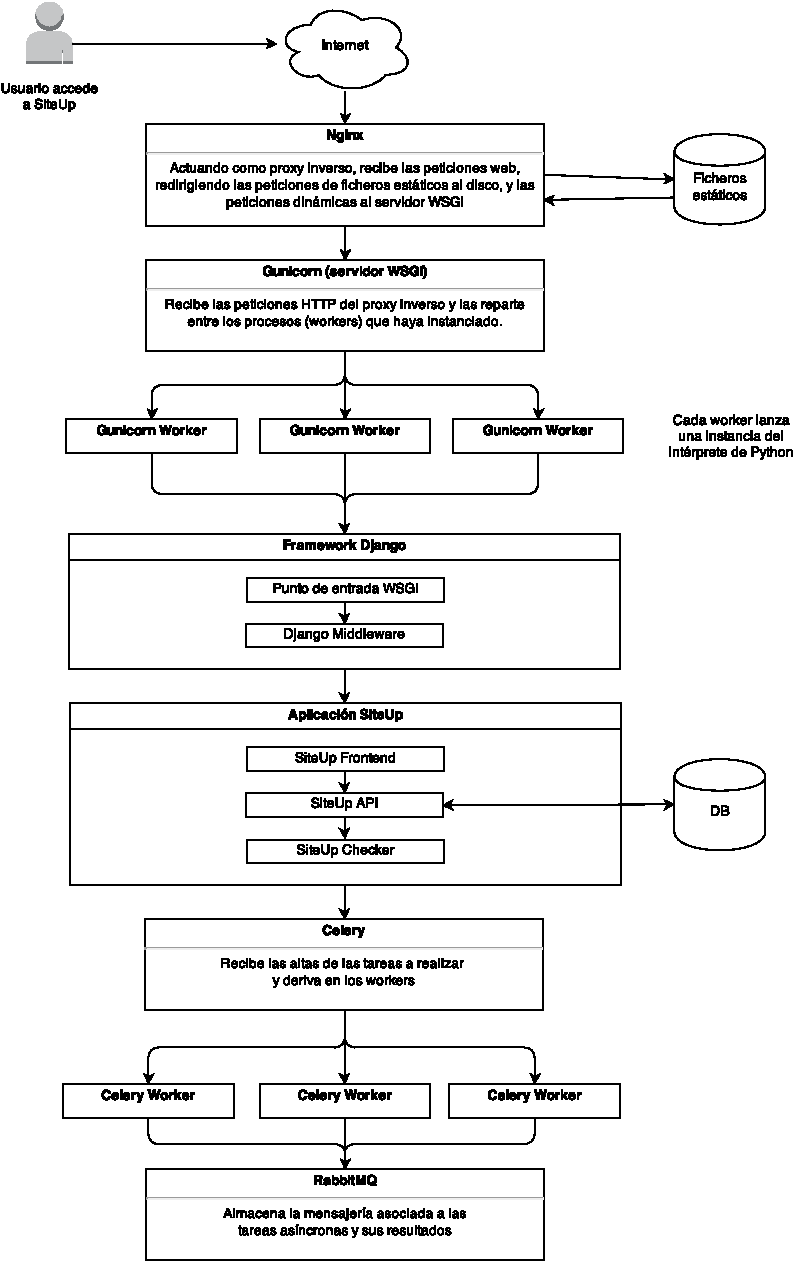
\includegraphics[width=0.9\textwidth]{5_diseno/diagrama_arquitectura_logica}
  \caption{Arquitectura lógica del sistema web}
  \label{fig:arquitectura-logica}
\end{figure}


\paragraph{Navegador}

Cuando un usuario desea acceder a SiteUp, abre un cliente web (habitualmente un
\textbf{navegador} web) y teclea la \ac{URL}. A partir de ahí, el navegador debe
obtener el contenido de la web. Para ello (ignorando cuestiones de bajo nivel,
como el envío de peticiones ARP o resoluciones de DNS) la acción fundamental es
hacer una \textbf{petición HTTP} al servidor que se encuentra en la URL
indicada. Esto se traduce en abrir una conexión TCP al puerto 80 del servidor
remoto y enviar unas cabeceras en las que se indique, entre otras cosas, qué
datos se quiere obtener.

\paragraph{Servidor proxy inverso}

En el servidor debe existir algún \textbf{servicio} que sea capaz de escuchar y
disponer peticiones en el puerto 80 del servidor (el número el puerto puede
variar). En nuestro caso el servidor deberá tener instalado \textbf{Nginx}, un
servidor web/proxy inverso que recibirá las peticiones HTTP del exterior. En
estas peticiones, enviadas por el navegador, se detalla qué recurso se necesita
enviar. 

En el caso de recursos estáticos, como por ejemplo ficheros de imágenes o
archivos de hojas de estilo en cascada (\ac{CSS}), es buena práctica que sea el
propio servidor el que sirva estos ficheros, dado que no necesitan de ningún
procesado dinámico, por lo que no tiene sentido desperdiciar recursos pasando la
petición al código Python.

En el caso de recursos dinámicos, esto es, las peticiones web a páginas
generadas dinámicamente, Nginx actuará de proxy inverso y pasará la petición al
manejador que se haya configurado. 

\paragraph{Servidor de aplicaciones Python}

Como se ha comentado, el proxy inverso ha detectado que hay una petición
dinámica y según su configuración la ha pasado al servidor de aplicaciones
Python. En el caso de nuestro proyecto se tratará del servidor
\textbf{Gunicorn}. Gunicorn sigue un model conocido como \textit{pre-fork
  worker}, que básicamente consiste en instanciar (\textit{forkear}) varios
procesos al lanzar el servidor que se encargarán de procesar las peticiones de
forma paralela, según el proceso padre las vaya repartiendo.

En el mundo del desarrollo web en Python se ha establecido un estándar, conocido
como \ac{WSGI}, que regula la forma en la que las aplicaciones web escritas en
Python se comunican con un servidor web. Por ello, cuando un worker recibe una
petición lo primero que hace es comunicarse con la interfaz WSGI de la
aplicación que se vaya a ejecutar, pasándole la petición y un puntero a un
\textit{callback} al que informar cuando la respuesta a la petición esté
lista. 

\paragraph{Punto de entrada WSGI}

Como se ha comentado, el worker del servidor de aplicaciones se comunica con la
interfaz WSGI. Todas las aplicaciones desarrolladas en Django cuentan con un
módulo \texttt{wsgi.py} que actúa como punto de entrada WSGI y que directamente
pasa la petición al \textit{middleware} de Django que empieza el procesamiento.

\paragraph{Middleware Django y aplicación}

A partir de este punto, la petición va rebotando entre código propio del
framework Django y código de la aplicación. El flujo habitual, en su forma más
básica es el siguiente:

\begin{enumerate}
\item Los módulos de \textit{middleware} que gestionan las peticiones reciben la
  petición actual.
\item Django revisa el fichero \texttt{urls.py} de la aplicación, que contiene
  una lista de URLs asociadas a funciones. Django compara la URL de la petición
  recibida y mira si coincide con alguna de las URLs del proyecto.
\item Si no hay coincidencia, Django devuelve una respuesta negativa,
  normalmente en forma de código de estado 404.
\item Si hay coincidencia, Django llama a la función asociada a esa URL --
  conocida como la \textbf{vista}. La vista procesa la petición, devolviendo una
  respuesta.
\item Esa respuesta hace el camino de forma inversa, pasando por todos los pasos
  hasta el cliente.
\end{enumerate}

Entrando más en detalle, una aplicación de Django se organiza en una
arquitectura de módulos pequeños o \textit{aplicaciones}, cada una de las cuales
debe tener una serire de responsabilidades reducida y acotada, de forma que sea
relativamente sencillo intercambiar las aplicaciones por otras. En el caso del
proyecto SiteUp, se cuenta con tres aplicaciones:

\begin{itemize}
\item \textbf{siteup\_frontend} gestiona las vistas de la aplicación, recibe las
  peticiones, muestra las páginas y gestiona formularios.

\item \textbf{siteup\_api} recibe las órdenes de \texttt{siteup\_frontend},
  haciendo los cambios necesarios en la base de datos, dando de alta las tareas
  y procesando resultados.

\item \textbf{siteup\_checker} cuenta con el código de bajo nivel para hacer los
  chequeos de diferentes tipos. Es principalmente una aplicación tipo
  \textit{helper}.

\end{itemize}

Cada aplicación en Django cuenta con una arquitectura de tres capas conocida
como \textbf{Modelo-Vista-Plantilla}, que se asimila al clásico patrón del
\textbf{Modelo-Vista-Controlador}.

\begin{itemize}
\item El \textbf{modelo} representa la información en la base de datos, evitando
  al usuario tener que utilizar código SQL. Para ello, Django cuenta con un
  \ac{ORM} que facilita el trabajo con registros de la base de datos.
\item Las \textbf{vistas} suelen ser funciones asociadas a una URL. La filosofía
  de Django es que las vistas sirvan solo como \textit{punto de paso} de los
  datos entre los modelos y las plantillas. Es mala práctica colocar lógica de
  negocio compleja en las vistas.
\item Las \textbf{plantillas} son la representación final de los datos, lo que
  acaba viendo el usuario. Las plantillas suelen estar escritas en HTML aunque
  pueden también representarse usando JSON, XML, etc.
\end{itemize}

La organización física de ficheros de un proyecto Django se ajusta perfectamente
a la organización lógica hasta ahora descrita, siendo habitual tener un árbol de
ficheros similar al siguiente:

\begin{itemize}
\item Raíz del proyecto
\item \texttt{siteup} --  Directorio de proyecto general.
  \begin{itemize}
  \item \texttt{settings.py} -- Configuración general.
  \item \texttt{urls.py} -- Configuración de URLs.
  \item \texttt{wsgi.py} -- Punto de acceso WSGI.
  \end{itemize}
\item \texttt{siteup\_api} --  Directorio para la app (suele haber más de uno).
  \begin{itemize}
  \item \texttt{views.py} -- Definición de vistas (funciones).
  \item \texttt{models.py} -- Definición de modelos.
  \item \texttt{tests.py} -- Definición de tests.
  \end{itemize}
\end{itemize}

Opcionalmente, las aplicaciones de Django pueden contar con ficheros
individuales para otros elementos, como formularios, mánagers, migraciones,
validadores, utilidades, filtros, procesadores de contexto, etcétera.

\paragraph{Servidor de tareas asíncronas}

Habrá peticiones en SiteUp cuyo objetivo sea dar de alta chequeos. Éstos dan
lugar a nuevas tareas que serán ejecutadas asíncronamente. Celery, el servidor
de tareas que se utiliza, cuenta con una arquitectura de \textit{workers}
similar a Gunicorn, que se reparten las tareas que son dadas de alta por
SiteUp. Estas tareas se ejecutan de forma periódica. 

Tras su conclusión, Celery se comunica con Django para dejar constancia de los
resultados de esas tareas en forma de modelos de la base de datos.

\paragraph{Broker de mensajes}

Por debajo de Celery se encuentra el \textit{bróker} de mensajes, que implementa
el ya mencionado estándar \ac{AMQP}. El bróker se encarga de almacenar las
tareas y sus resultados en forma de mensajes en una cola. 

En este proceso es necesario \textit{traducir} las tareas a un formato que sea
almacenable y gestionable en una cola. En el caso de Django lo más habitual es
utilizar Pickle, el estándar de facto para la serialización de objetos Python.

\subsubsection{Aplicación Android}
\label{subsec:arquitectura-logica-android}


\begin{figure}[hbtp]
  \centering
  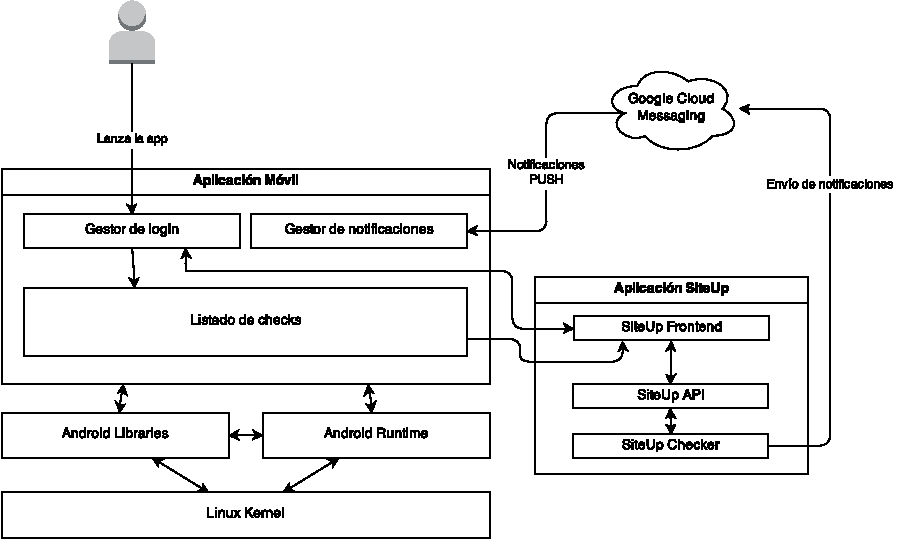
\includegraphics[width=\textwidth]{5_diseno/diagrama_arquitectura_logica_android}
  \caption{Arquitectura lógica de la aplicación Android}
  \label{fig:arquitectura-logica-android}
\end{figure}

En la figura~\ref{fig:arquitectura-logica-android} se puede ver un esquema
general de la arquitectura de la aplicación móvil desarrollada para el sistema
operativo Android. El flujo se detalla a continuación:

\paragraph{Lanzador}

Partimos de la premisa de que el usuario ha instalado la aplicación
\textit{SiteUp Client} en su dispositivo. Si el usuario decide lanzar la
aplicación, deberá dirigirse al lanzador de aplicaciones de su dispositivo y
pulsar sobre el icono de la aplicación, con lo que se iniciará la ejecución.

\paragraph{Gestor de inicio de sesión}

Cuando la aplicación Android se inicia, se lanza una actividad
\texttt{LoginActivity} que hace varias cosas. En primer lugar, verifica si hay
datos de inicio de sesión guardados en el dispositivo. Si no los hay, muestra un
formulario para que el usuario introduzca su nombre de usuario y contraseña. 

Una vez obtenidos los datos, la aplicación móvil se comunica con la plataforma
web para verificar el inicio de sesión. En caso correcto, la plataforma web
envía la información de los chequeos a la aplicación móvil.

\paragraph{Listado de chequeos}

En la aplicación móvil se ha dispuesto una actividad \texttt{CheckListActivity}
que mostrará la lista de chequeos que el usuario ha dado de alta, con
información básica de cada uno de ellos. Cuando el usuario pulse en cualquiera
de los chequeos, se abrirá un navegador y será redirigido a la plataforma web,
particularmente a la página de detalle del chequeo seleccionado.

\paragraph{Gestor de notificaciones}

La aplicación móvil cuenta con un servicio capaz de recibir notificaciones
\textit{Push} del servicio \textit{Google Cloud Messaging}. Cuando se recibe un
mensaje, se muestra una notificación al usuario, informándole también de forma
audible y a través de vibración. La notificación aparece en el área de
notificaciones del sistema operativo. Si el usuario pulsa en la notificación
podrá obtener información sobre el chequeo involucrado.

\paragraph{Google Cloud Messaging}

GCM~\cite{gcm} es un servicio para Android que permite enviar datos desde un
servidor a los dispositivos Android que tengan instaladas una aplicación en
particular. El servicio GCM se encarga de todos los aspectos de la entrega de
mensajes. Se trata de un servicio gratuito independientemente del número de
mensajes y el tamaño de éstos.

GCM recibirá las notificaciones del \textit{backend} de la plataforma móvil, y
se encargará de reenviarlas a los dispositivos Android.

\paragraph{SiteUp Checker}

Dentro de la aplicación móvil, el módulo \texttt{siteup\_checker} es el
encargado de realizar los chequeos, y también de enviar las notificaciones a los
dispositivos Android a través del servicio GCM. La plataforma web tiene una
clave especial con la que se realizan las peticiones a los servidores de Google,
enviando los mensajes.

\paragraph{Runtime y bibliotecas de Android}

Las aplicaciones Android utilizan como base el runtime y las bibliotecas que
provee el sistema operativo para acceder a las funciones del dispositivo y demás
servicios, como la comunicación por red, acceso a datos del usuario, lectura y
escritura de ficheros en el dispositivo, etcétera.


\section{Diseño físico de datos}
\label{sec:diseno-fisico-datos}

En la figura~\ref{fig:diagrama-modelos} se muestra el diagrama de modelos que se
reflejará en la base de datos, donde se puede apreciar cada una de las tablas
que forman el proyecto, así como los campos de las tablas y las relaciones entre
ellas.

\begin{figure}[htbp]
  \centering
  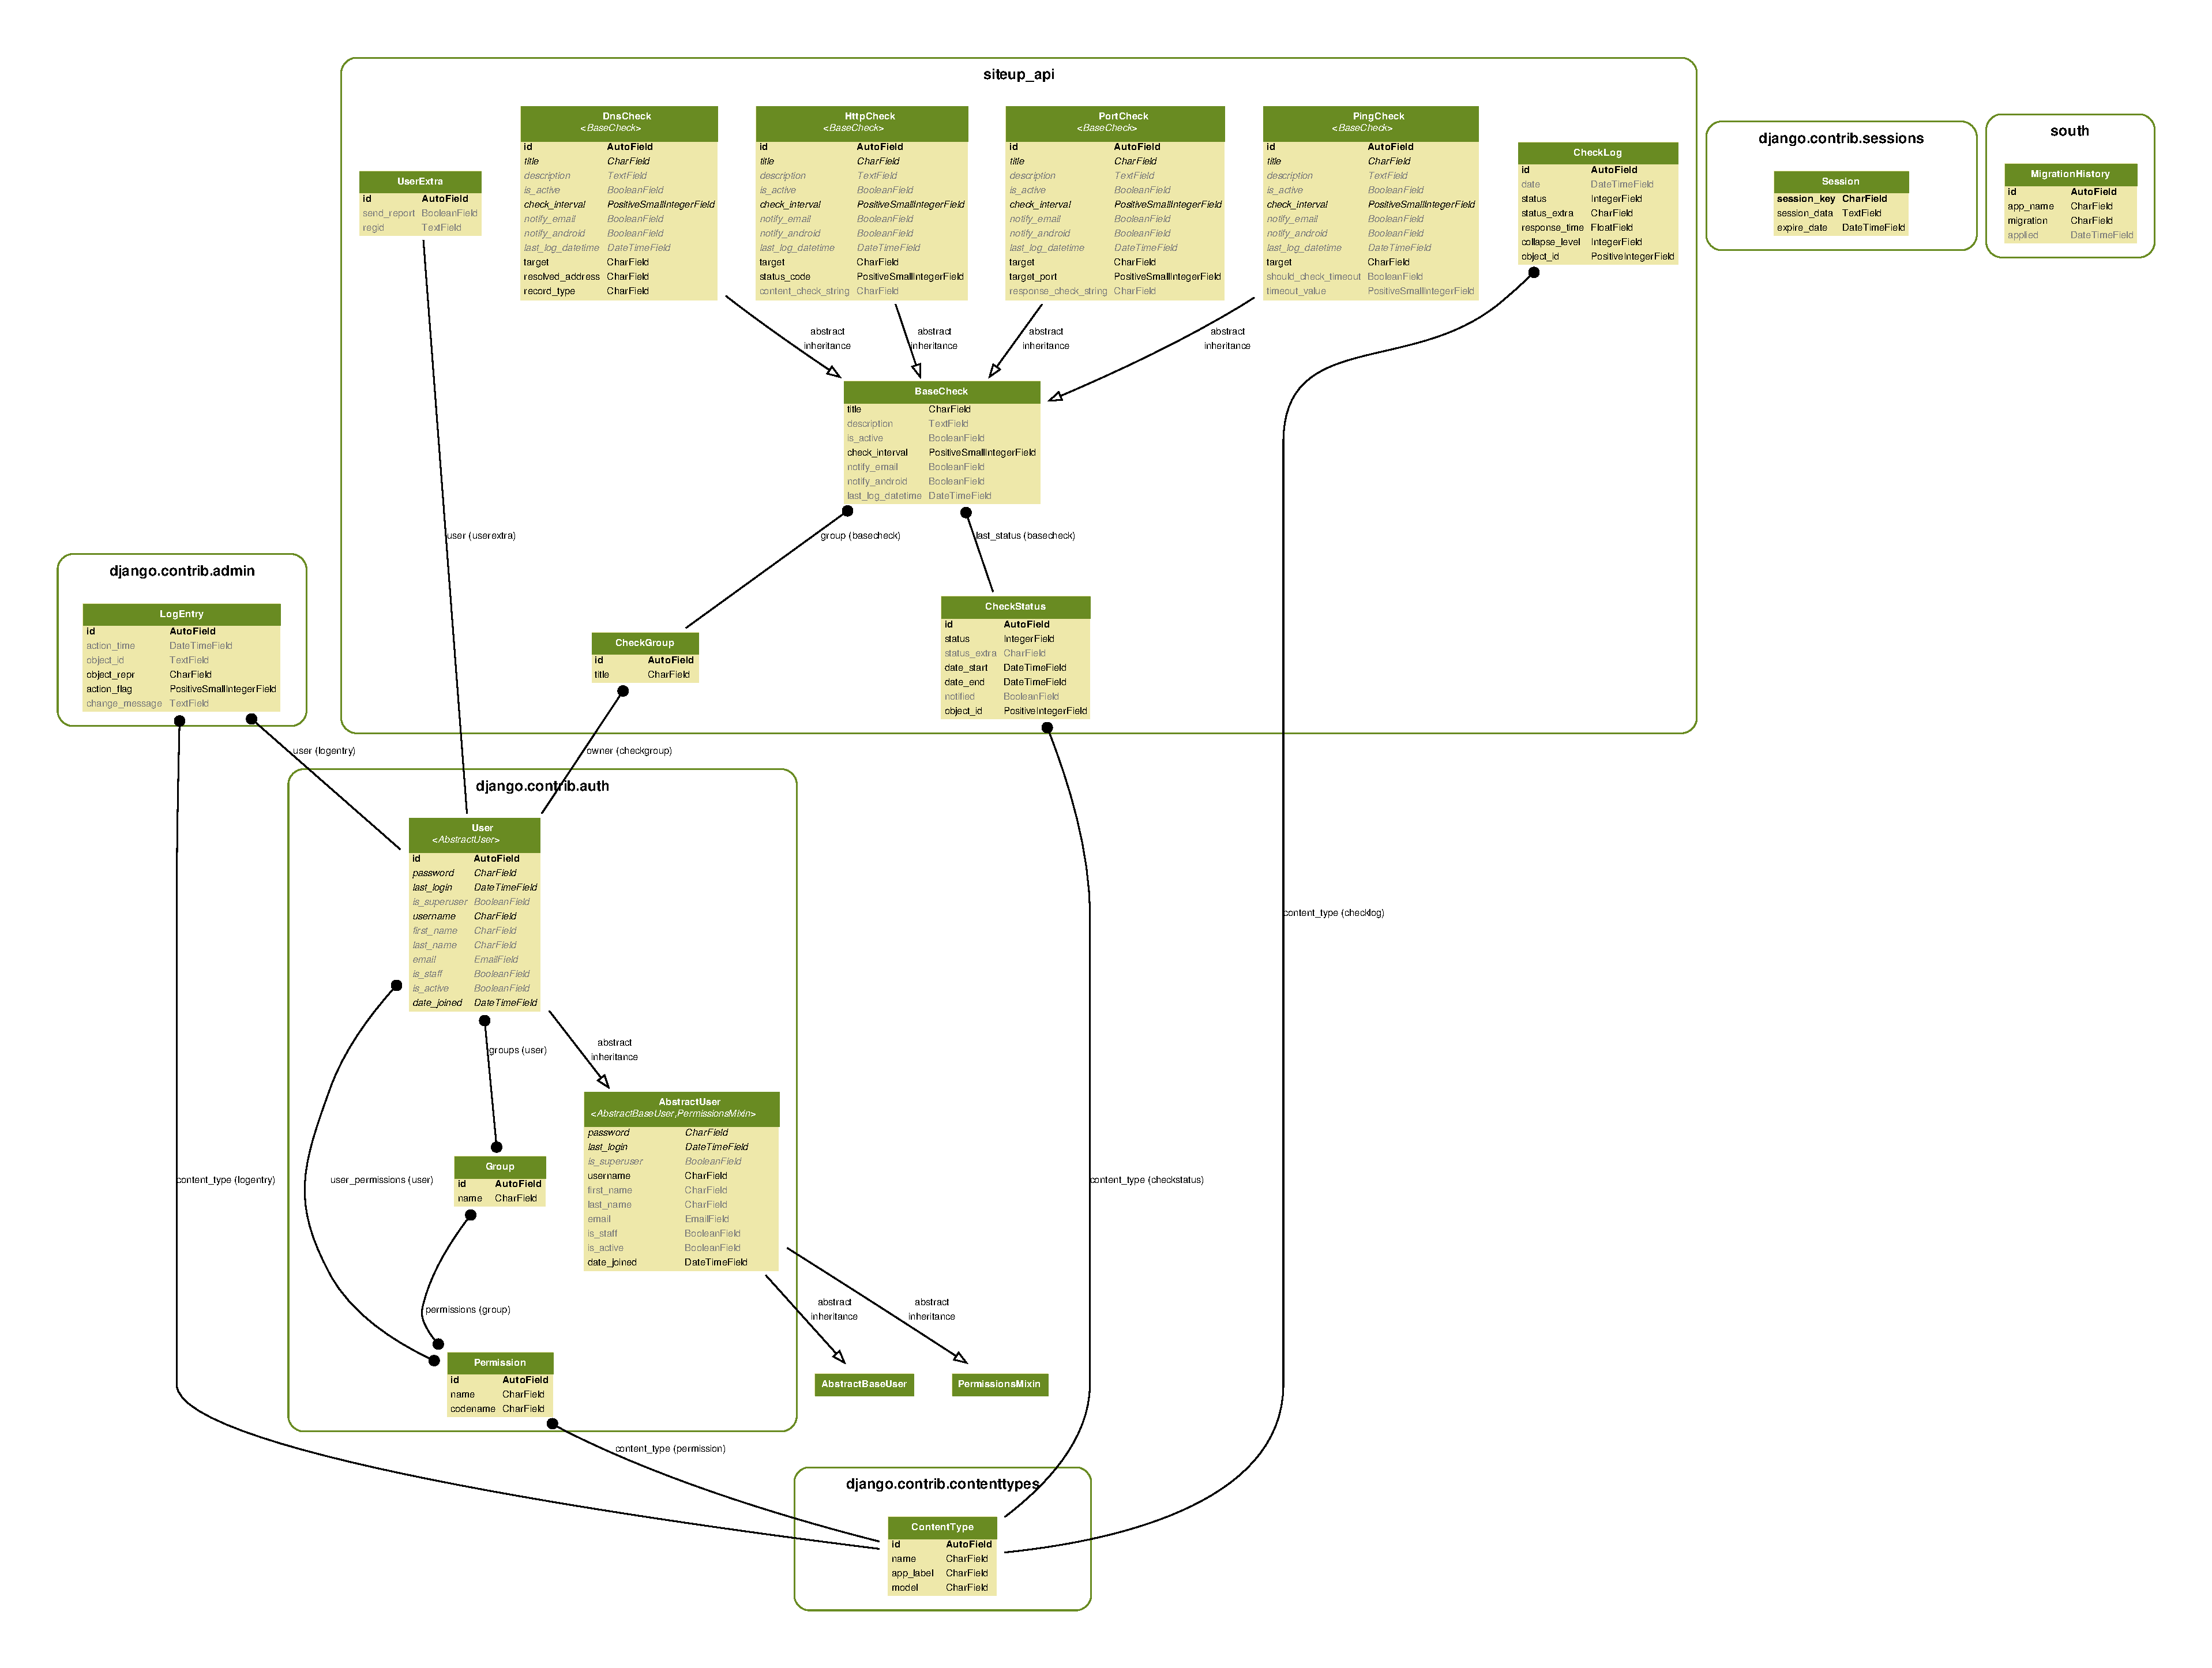
\includegraphics[angle=90, width=\textwidth]{5_diseno/diagrama-modelos}
  \caption{Diseño de la base de datos}
  \label{fig:diagrama-modelos}
\end{figure}

El diseño de los datos se ha hecho mediante las herramientas de mapeo
objeto-relacional que ofrece el framework Django. A continuación se detallan los
principales modelos con los que cuenta el sistema.

\subsection{User}

Este modelo representa a un usuario registrado en el sistema. Es un modelo
predeterminado de Django y forma parte de la aplicación \texttt{django.contrib.auth}.

Sus principales campos son:

\begin{itemize}
\item \texttt{username} - Nombre de usuario.
\item \texttt{password} - Contraseña. Se almacena en forma de cifrado
  irreversible de acuerdo a las exigencias de la actual Ley de Protección de Datos.
\item \texttt{email} - Dirección de correo electrónico.
\end{itemize}

\subsection{UserExtra}

Este modelo guarda información adicional sobre los usuarios, evitando así tener
que modificar el modelo que integra Django. Forma parte de la aplicación \texttt{siteup\_api}.

Sus principales campos son:

\begin{itemize}
\item \texttt{send\_report} - Booleano, indica si el usuario recibirá reportes
  diarios sobre el estado de sus chequeos.
\item \texttt{regid} - Texto, guarda el identificador único del dispositivo
  Android obtenido a través de Google Play Services.
\end{itemize}

\subsection{CheckGroup}

Parte de la aplicación \texttt{siteup\_api}. Identifica a un grupo de
chequeos. Todos los chequeos deben pertenecer a un grupo. 

El campo principal de este modelo es \texttt{title}, que guarda una cadena con
el título del grupo.

\subsection{BaseCheck}

Parte de la aplicación \texttt{siteup\_api}. Este modelo \textbf{abstracto}
guarda campos comunes a todos los tipos de chequeos. No tiene representación
directa en la base de datos, sino que sirve para evitar duplicidad de código.

Sus principales campos son:

\begin{itemize}
\item \texttt{title} - Texto, representa el título del chequeo.
\item \texttt{description} - Texto, representa la descripción del chequeo.
\item \texttt{is\_active} - Booleano, indica si el chequeo está activo.
\item \texttt{check\_interval} - Entero, indica el intervalo entre chequeos en minutos.
\item \texttt{notify\_email} - Booleano, indica si los cambios de estado del
  chequeo se notificarán vía correo electrónico.
\item \texttt{notify\_android} - Booleano, indica si los cambios de estado del
  chequeo se notificarán vía Android utilizando notificaciones push.
\item \texttt{last\_log\_datetime} - Fecha, almacena la fecha de la última vez que se lanzó el chequeo.
\end{itemize}

\subsection{DnsCheck}

Parte de la aplicación \texttt{siteup\_api}. Este modelo deriva de
\texttt{BaseCheck} y representa un chequeo de registros DNS. Sus principales campos son:

\begin{itemize}
\item \texttt{target} - Texto, indica el dominio a chequear.
\item \texttt{record\_type} - Enum, indica el tipo de registro a chequear. Puede ser de tipo A, AAAA, CNAME, MX y TXT.
\item \texttt{resolved\_address} - Texto, indica el contenido que debe tener el registro revisado.
\end{itemize}

\subsection{HttpCheck}

Parte de la aplicación \texttt{siteup\_api}. Este modelo deriva de
\texttt{BaseCheck} y representa un chequeo a través de peticiones HTTP.

Sus principales campos son:

\begin{itemize}
\item \texttt{target} - Texto, indica la URL a comprobar.
\item \texttt{status\_code} - Entero, indica el código de estado que se debe recibir.
\item \texttt{content\_check\_string} - Cadena, representa una cadena de texto
  que, opcionalmente, debe estar presente en la respuesta obtenida desde la URL indicada.
\end{itemize}

\subsection{PortCheck}

Parte de la aplicación \texttt{siteup\_api}. Este modelo deriva de
\texttt{BaseCheck} y representa un chequeo de puertos remotos.

Sus principales campos son:

\begin{itemize}
\item \texttt{target} - Cadena, identifica el servidor remoto al que conectarse.
\item \texttt{target\_port} - Entero, indica el puerto remoto al que conectarse.
\item \texttt{response\_check\_string} - Cadena, representa una cadena de texto
  que, opcionalmente, debe estar presente en la respuesta obtenida desde el servidor.
\end{itemize}

\subsection{PingCheck}

Parte de la aplicación \texttt{siteup\_api}. Este modelo deriva de
\texttt{BaseCheck} y representa un chequeo mediante el envío de paquetes \ac{ICMP}.

Sus principales campos son:

\begin{itemize}
\item \texttt{target} - Cadena, identifica al servidor remoto que hay que chequear.
\item \texttt{should\_check\_timeout} - Booleano, indica si hay que comprobar el tiempo de respuesta de los paquetes ping.
\item \texttt{timeout\_value} - Entero, si el anterior campo evalúa a
  \textit{Verdadero}, este campo guarda el tiempo de respuesta máximo permitido.
\end{itemize}

\subsection{CheckLog}

Parte de la aplicación \texttt{siteup\_api}. Es un registro (\textit{log}) que
representa el resultado de ejecutar un chequeo.

Sus principales campos son:

\begin{itemize}
\item \texttt{date} - Fecha, representa el momento en el que se obtuvo el resultado.
\item \texttt{status} - Entero, representa el estado del chequeo que se ha
  obtenido. Los posibles valores son:
  \begin{itemize}
  \item 0: el chequeo ha terminado correctamente y el estado es correcto (\textit{Up}).
  \item 1: el chequeo ha terminado correctamente y el estado es negativo (\textit{Down}).
  \item 2: el chequeo no ha podido concluirse. Equivalente en estadísticas al estado negativo. (\textit{Error}).
  \end{itemize}
\item \texttt{response\_time} - Entero, solo válido para los chequeos de tipo
  Ping. Guarda el tiempo de respuesta obtenido.
\item \texttt{collapse\_level} - Entero. Indica el nivel de \textit{colapsado}
  del registro. Dado que el número de registros es muy alto (en una hora pueden
  llegar a generarse más de 3600 registros por chequeo), es necesario resumir
  los registros más antiguos. Este campo indica si el \textit{CheckLog} ya ha
  sido resumido o no.
\end{itemize}

\subsection{CheckStatus}

Parte de la aplicación \texttt{siteup\_api}. Representa un cambio de estado de
un chequeo. Cuando un chequeo es ejecutado, se genera una instancia de
\textit{CheckLog} y se comprueba el estado de éste con el estado de la última
comprobación. Si se verifica que el estado ha cambiado con respecto a los
últimos estados, se genera una instancia de \textit{CheckStatus} y se lanzan las
notificaciones pertinentes.

Los campos principales de este modelo son:

\begin{itemize}
\item \texttt{status} - Entero, indica el estado. El código numérico responde al
  mismo formato que se sigue en el modelo \textit{CheckLog}.
\item \texttt{status\_extra} - Cadena, guarda información adicional sobre el estado.
\item \texttt{date\_start} - Fecha, indica el momento en el que el chequeo
  cambia a este estado.
\item \texttt{date\_end} - Fecha, indica el momento en el que el chequeo deja de
  estar en este estado. Si es el estado actual de un chequeo, se mantiene en blanco.
\item \texttt{notified} - Booleano, indica si este cambio de estado ha sido ya notificado.

\end{itemize}

\subsection{Session}

Parte de la aplicación \texttt{django.contrib.sessions}. Representa una sesión
de usuario en la aplicación web. Sus campos principales son:

\begin{itemize}
\item \texttt{session\_key} - Cadena, guarda el identificador de la sesión.
\item \texttt{session\_data} - Texto, guarda los datos asociados a la sesión.
\item \texttt{expire\_date} - Fecha, indica hasta qué fecha son válidos los
  datos de la sesión.
\end{itemize}

\subsection{MigrationHistory}

Parte de la aplicación \texttt{south}. Representa una migración de la base de
datos. Los campos principales son:

\begin{itemize}
\item \texttt{app\_name} - Cadena, nombre de la app sobre la que se ahce la migración.
\item \texttt{migration} - Cadena, identificador de la migración.
\item \texttt{applied} - Fecha, indica cuándo se aplicó la migración.
\end{itemize}

\subsection{ContentType}

Parte de la aplicación \texttt{django.contrib.contenttypes}. Es el bloque
principal del \textit{Content Types Framework}, un framework integrado en Django
que permite trabajar de forma genérica con los modelos, ofreciendo
funcionalidades como la posibilidad de crear claves foráneas genéricas (es
decir, que puedan apuntar a cualquier modelo. 

Una instancia de \textit{ContentType} representa un modelo particular de una
aplicación en concreto. Los campos que contiene son:

\begin{itemize}
\item \texttt{name} - Cadena, nombre del modelo en formato legible.
\item \texttt{model} - Cadena, nombre original del modelo.
\item \texttt{app\_label} - Cadena, nombre de la aplicación a la que pertence el
  módulo.
\end{itemize}

\section{Diseño de la imagen corporativa}

La \textbf{imagen corporativa} del proyecto comprende el diseño del
\textbf{logotipo}, la elección de la paleta de \textbf{colores} y las
\textbf{tipografías}, que se usan en el diseño de la web, emails y cualquier
otro elemento visual.

Para su elaboración se han seguido ciertas premisas o \textit{guías de
  branding}, de forma que se consiguiese el look más adecuado:

\begin{itemize}
\item \textbf{Diseño minimalista}. En SiteUp, la información es lo más
  importante, así que no tiene sentido utilizar un diseño muy sobrecargado.
\item \textbf{Colores monocromáticos}. Siguiendo en la línea del punto anterior,
  esta \textit{regla} facilita que haya una consistencia en las interfaces de la
  web y la aplicación móvil sin tener que recurrir a complejas combinaciones de
  color.
\item \textbf{Tipografías libres}. Era importante no utilizar tipografías que
  requiriesen una licencia comercial para su uso.
\end{itemize}

\subsection{Diseño del logotipo}
\label{subsec:logotipo}

Partiendo del nombre del proyecto se pensaron varios bocetos para el
logotipo. La idea principal era jugar con las dos palabras que componen el
nombre: \textit{Site} y \textit{Up}. Para la primera palabra, la metáfora de
usar una ventana de un navegador o algo que representase un servidor era
demasiado compleja, así que se decidió simplemente usar la letra S. 

Por otro lado, para la segunda palabra estaba claro desde el principio que se
usaría alguna metáfora de tipo flecha para representar la dirección
\textit{arriba}. Se probaron distintos tipos de flechas y al final se decidió
por una doble flecha de tipo galón, con suficiente separación para que se viese
en bajas resoluciones. El logotipo resultante se puede ver en la
figura~\ref{fig:logotipo}

\begin{figure}[H]
  \centering
  
\includegraphics[width=0.5\textwidth]{5_diseno/logo.png}
  \caption{Logotipo de SiteUp}
  \label{fig:logotipo}
\end{figure}

\subsection{Elección de la gama cromática}

Teniendo en mente la idea apuntada anteriormente de que la gama de colores
debería ser preferiblemente monocromática, se empezó a buscar un tono que
funcionase con la temática del sitio. Se hizo una búsqueda de sitios web de
servicios de soporte, y en la mayoría de ellos la gama cromática era siempre muy
neutra, con tonos poco saturados y casi siempre fríos.

\begin{figure}[H]
  \centering
  
\includegraphics[width=\textwidth]{5_diseno/paleta-colores}
  \caption{Detalle de la paleta de colores de SiteUp}
  \label{fig:colores}
\end{figure}

Así, tras varias pruebas, se decidió optar por una gama de azules poco
saturados, rozando el grisáceo. En la figura~\ref{fig:colores} se detalla la
paleta de colores principal.

\subsection{Elección de la tipografía}

Siguiendo las directrices apuntadas previamente, se buscaba una tipografía
sencilla y minimalista. Se probaron algunas alternativas comerciales, empezando,
cómo no, por Helvética y pasando por Myriad Pro, Próxima Nova y algunas
otras. Al final nos decantamos por utilizar \textbf{Open Sans}~\cite{open-sans},
una tipografía sans-serif limpia y moderna, de corte humanista, y desarrollada
por Steve Matteson para Google.

Se trata de una tipografía limpia, optimizada para la legibilidad en toda clase
de soportes, y por supuesto libre, bajo una licencia Apache 2.0.

\begin{figure}[H]
  \centering
  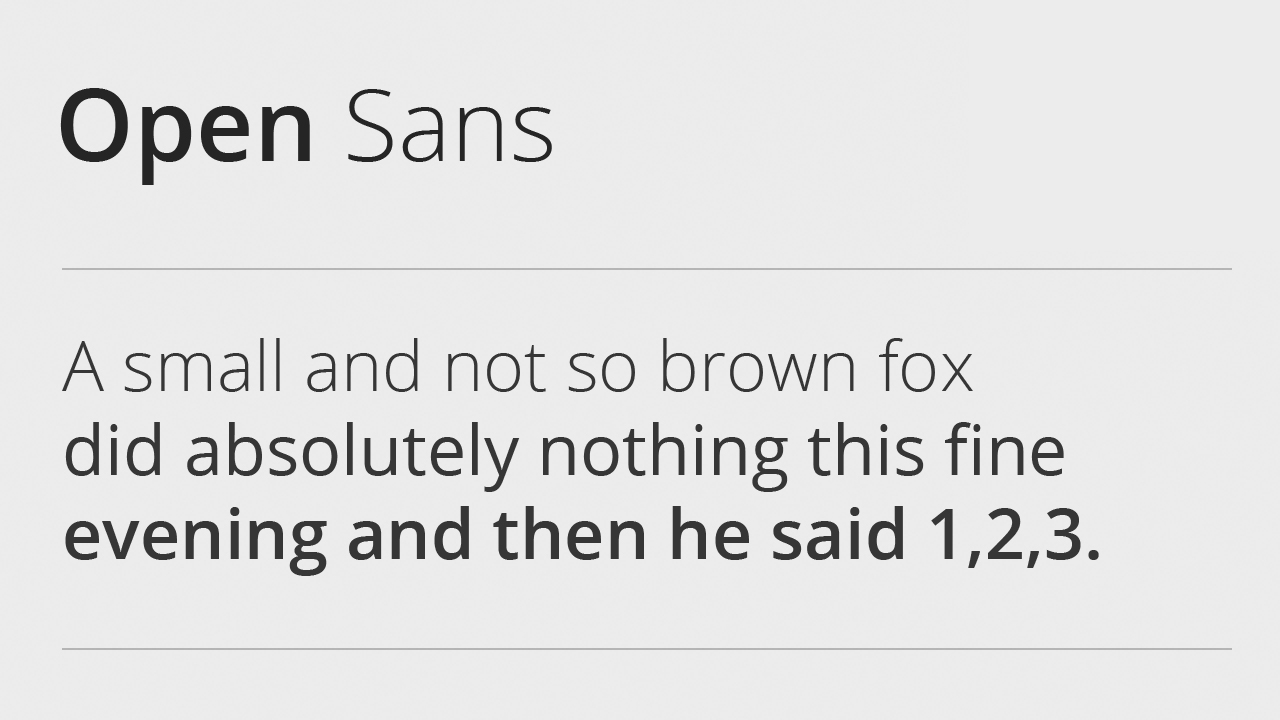
\includegraphics[width=0.8\textwidth]{5_diseno/open-sans}
  \caption{Muestra de Open Sans en diferentes pesos}
\end{figure}

\section{Diseño de la interfaz de usuario de la plataforma web}

En esta sección se detallarán las interfaces visuales de la plataforma web del
proyecto, indicando qué acciones realizan cada uno de los componentes que las
conforman.

\subsection{Pantalla de inicio}

\begin{figure}[htbp]
  \centering
  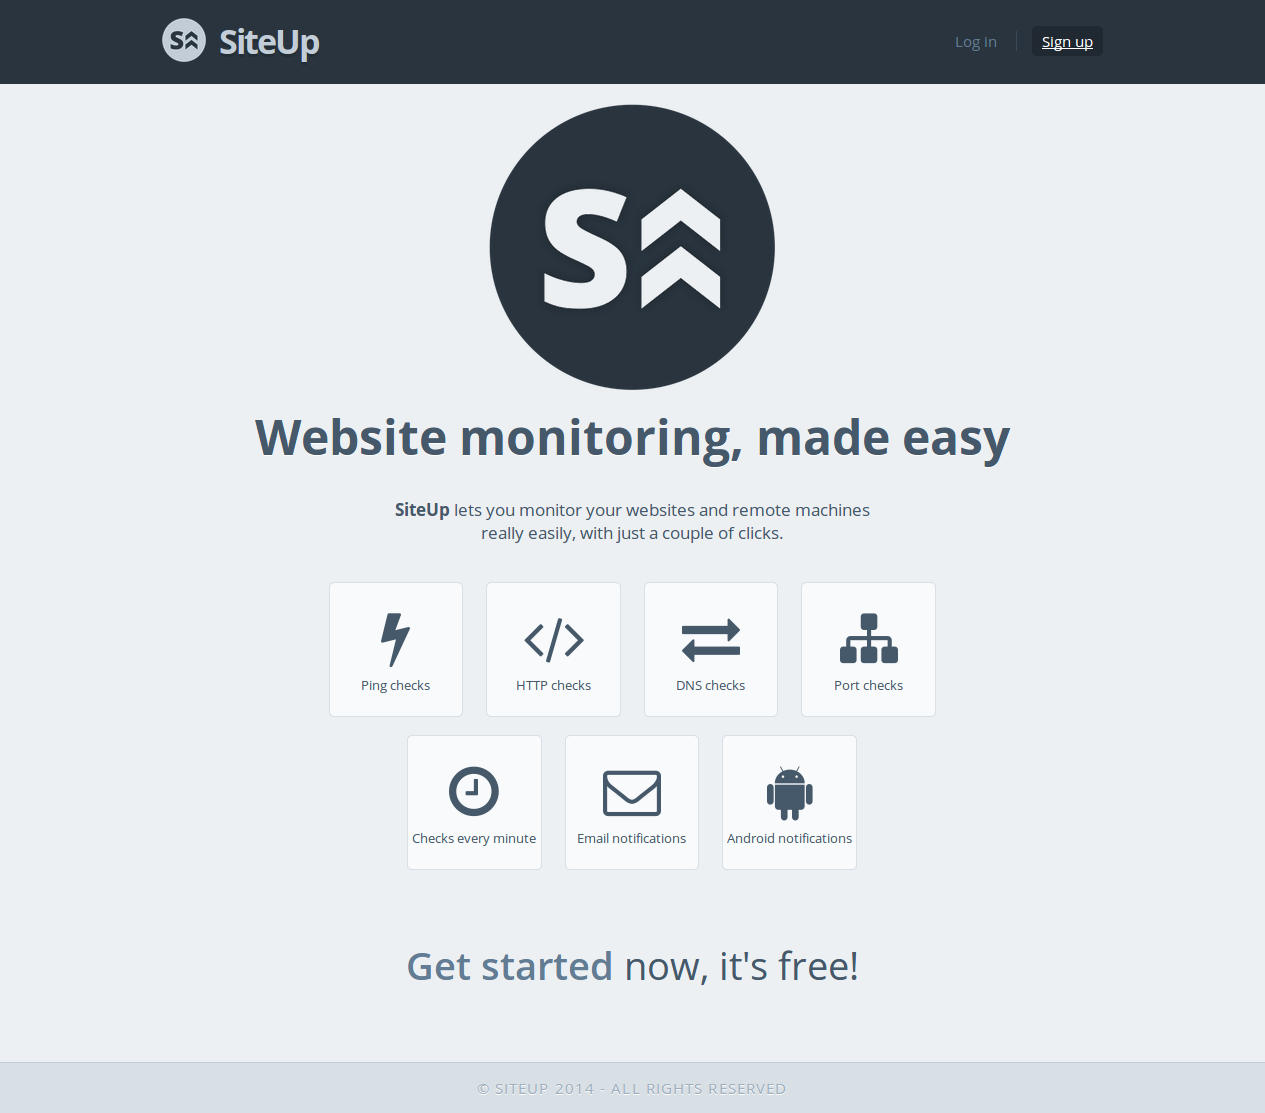
\includegraphics[width=\textwidth]{5_diseno/web-home.png}
  \caption{Pantalla de inicio}
  \label{fig:web-home}
\end{figure}

En la figura~\ref{fig:web-home} se ve el diseño de página de inicio, o
\textit{home}, de la plataforma web. Es la pantalla que aparece al acceder a la
base del proyecto. Se componen de una barra superior de navegación en la que
aparece el logotipo a la izquierda, y las opciones de navegación a la
derecha. Al pulsar el logotipo, se redirige a la pantalla de inicio.

Si el usuario no está logueado, las opciones de navegación disponibles son:

\begin{itemize}
\item \textbf{Log in}: lleva al usuario a la pantalla de inicio de sesión.
\item \textbf{Sign up}: lleva al usuario a la pantalla de registro de usuario.
\end{itemize}

Si el usuario sí está logueado, las opciones que aparecen son diferentes:

\begin{itemize}
\item \textbf{Dashboard}: lleva al usuario al listado de chequeos.
\item \textbf{Your profile}: lleva al usuario al formulario de datos personales.
\item \textbf{Log out}: cierra la sesión del usuario.
\end{itemize}

La barra de navegación superior tiene el mismo comportamiento en todas las
secciones de la web.


\subsection{Pantalla de inicio de sesión}

\begin{figure}[htbp]
  \centering
  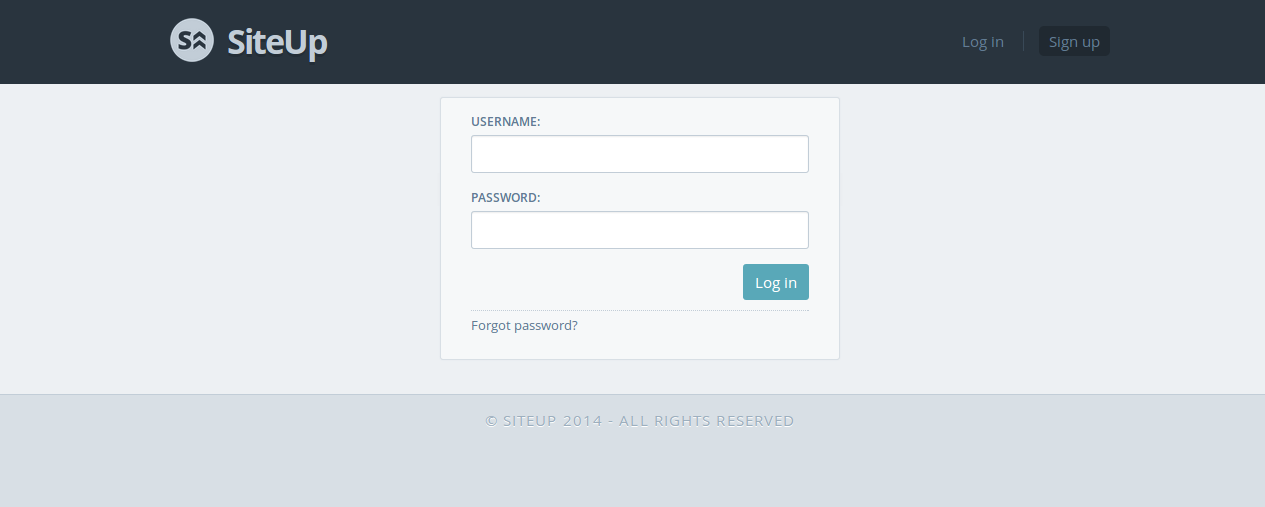
\includegraphics[width=\textwidth]{5_diseno/web-login.png}
  \caption{Pantalla de inicio de sesión}
  \label{fig:web-login}
\end{figure}

En la figura~\ref{fig:web-login} se ve el diseño de la pantalla de inicio de
sesión. Se presenta un formulario en el que el usuario deberá escribir su nombre
de usuario y su contraseña, y tras ello pulsar el botón de \textit{Login}. En
caso de que los datos introducidos sean correctos, el sistema iniciará sesión y
redirigirá al usuario a la lista de chequeos. En caso contrario, volverá a
aparecer el formulario con los errores que se hayan producido.

Opcionalmente, si el usuario no recuerda su contraseña puede pulsar en el botón
de \textit{Forgot password?}, lo que le llevará a la pantalla de recuperación de
contraseña.

\subsection{Pantalla de recuperación de contraseña}

\begin{figure}[htbp]
  \centering
  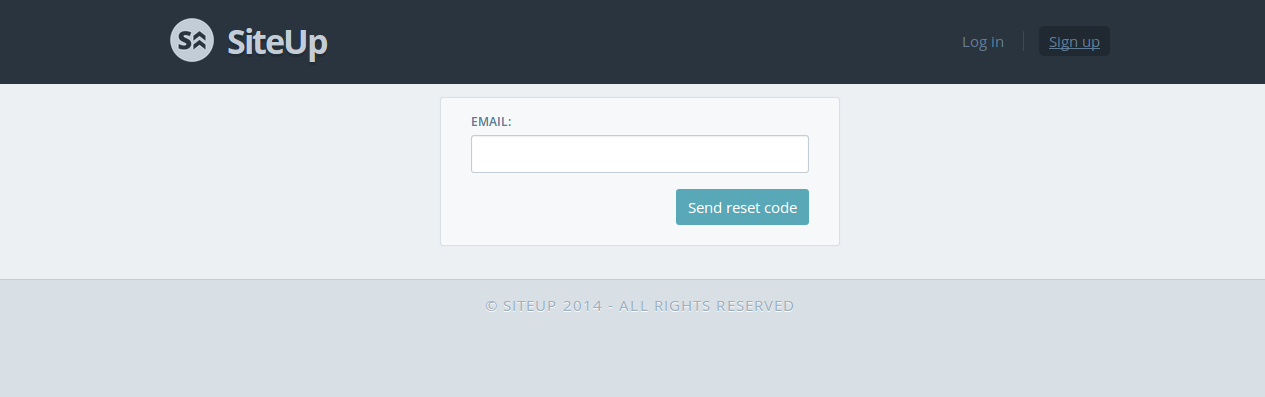
\includegraphics[width=\textwidth]{5_diseno/web-forgot-password}
  \caption{Pantalla de recuperación de contraseña}
  \label{fig:web-forgot-password}
\end{figure}

En esta pantalla, visible en la figura~\ref{fig:web-forgot-password}, el usuario
podrá introducir su correo electrónico para recuperar su contraseña. Tras
rellenar el campo de texto, deberá pulsar el botón. Si el email introducido es
correcto, el sistema enviará un correo electrónico con instrucciones para
reiniciar la contraseña, y en pantalla se mostrará un mensaje indicando que se
ha iniciado el proceso de reinicio.

% \vfill

\subsection{Pantalla de registro de usuario}

En la figura~\ref{fig:web-register} se puede ver la pantalla de registro de
usuario.

\begin{figure}[htbp]
  \centering
  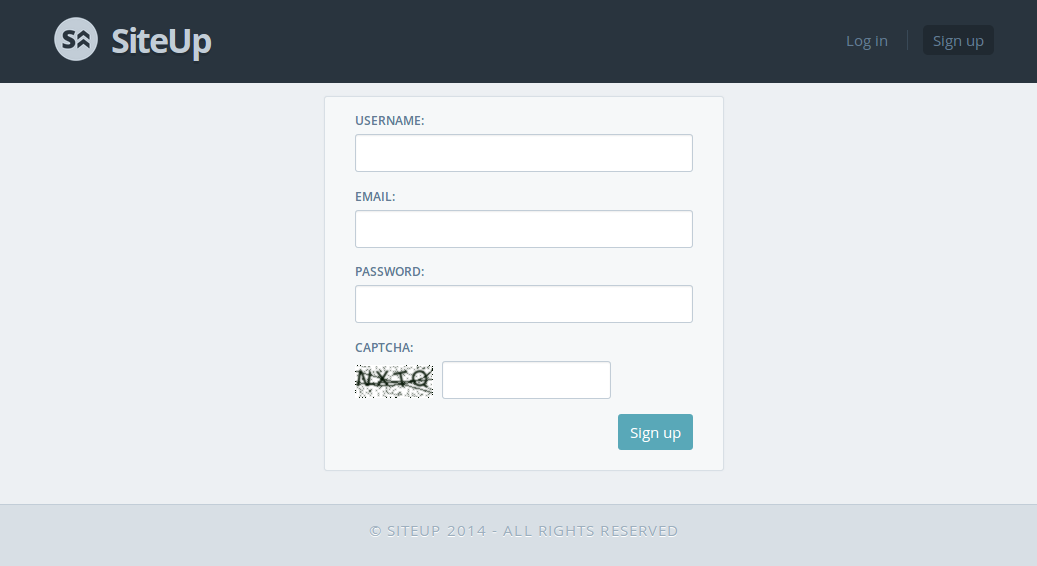
\includegraphics[width=\textwidth]{5_diseno/web-register}
  \caption{Pantalla de registro de usuario}
  \label{fig:web-register}
\end{figure}

Dispone de un formulario, en el que el usuario deberá introducir sus datos
personales: nombre de usuario, dirección de correo electrónico y contraseña. Una
vez rellenos, deberá pulsar el botón. Si los datos son correctos, el sistema
creará la cuenta de usuario. Si no, el sistema volverá a mostrar el formulario,
resaltando los errores en los datos.

% \vfill

\subsection{Pantalla de lista de chequeos}

\begin{figure}[htbp]
  \centering
  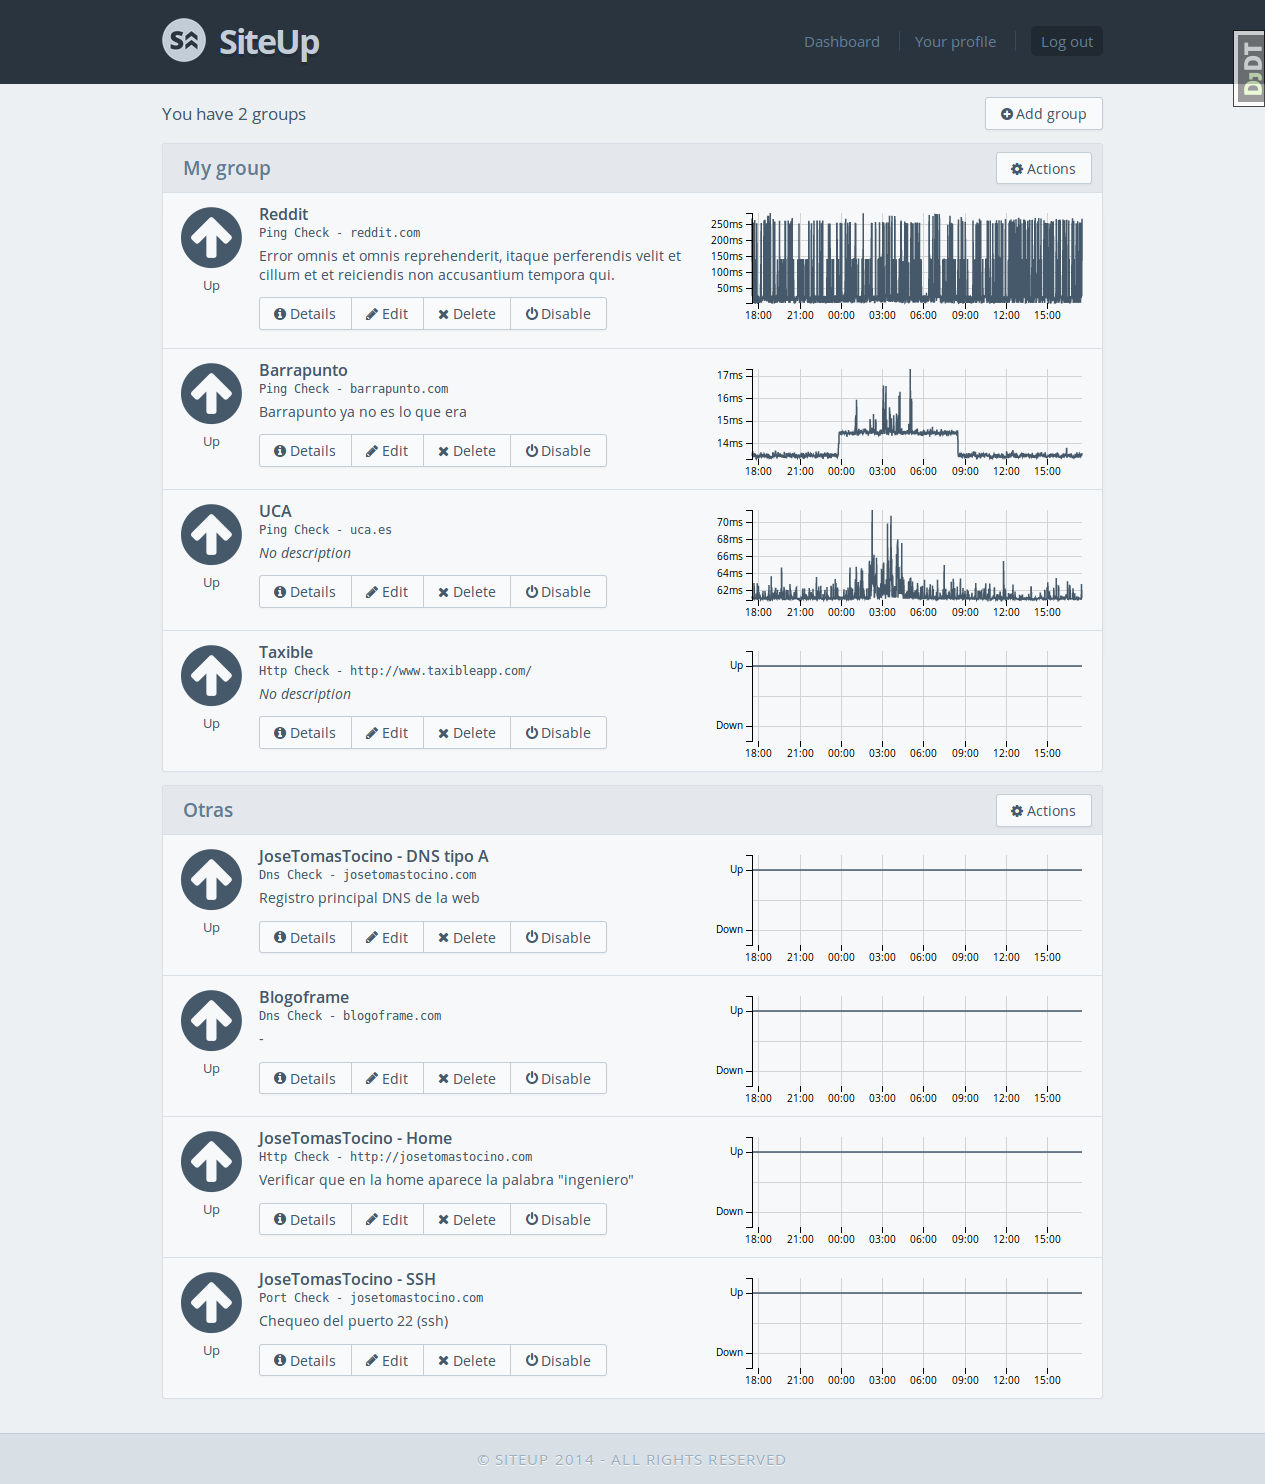
\includegraphics[width=\textwidth]{5_diseno/web-dashboard}
  \caption{Pantalla de lista de chequeos}
  \label{fig:web-dashboard}
\end{figure}

En la figura~\ref{fig:web-dashboard} se puede ver la pantalla principal de
SiteUp, la lista de chequeos o \textbf{dashboard}. En esta pantalla aparecen los
grupos de chequeos que tiene dados de alta un usuario, así como los chequeos que
pertenecen a cada grupo. Desde esta pantalla se pueden hacer un gran número de
operaciones:

\begin{itemize}
\item Pulsando el botón \textit{Add group} aparecerá la pantalla de creación de
  grupo.
\item Cada grupo tiene un menú desplegable que aparece al pulsar o colocar el
  ratón sobre el botón \textit{Actions}. Desde ahí, es posible:
  \begin{itemize}
  \item Añadir un chequeo al grupo pulsando el botón \textit{Add check}.
  \item Activar todos los chequeos del grupo pulsando el botón \textit{Enable
      all checks}.
  \item Desactivar todos los chequeos del grupo pulsando el botón
    \textit{Disable all checks}.
  \item Editar los detalles del grupo pulsando el botón \textit{Edit}.
  \item Borrar el grupo y los chequeos que contiene pulsando el botón \textit{Delete}.
  \end{itemize}
\item Dentro de cada grupo aparece cada uno de los chequeos que contiene, con un
  icono indicando el estado del chequeo, el título, descripción, una gráfica de
  su estado en las últimas 24 horas y una serie de botones de acción, que
  permiten:
  \begin{itemize}
  \item Ver los detalles del chequeo pulsando el botón \textit{Details}.
  \item Editar las propiedades del chequeo con el botón \textit{Edit}.
  \item Borrar el chequeo con el botón \textit{Delete}.
  \item Activar o desactivar el chequeo pulsando \textit{Enable} o
    \textit{Disable}.
  \end{itemize}

\end{itemize}

% \vfill

\subsection{Pantalla de creación de grupo}

\begin{figure}[htbp]
  \centering
  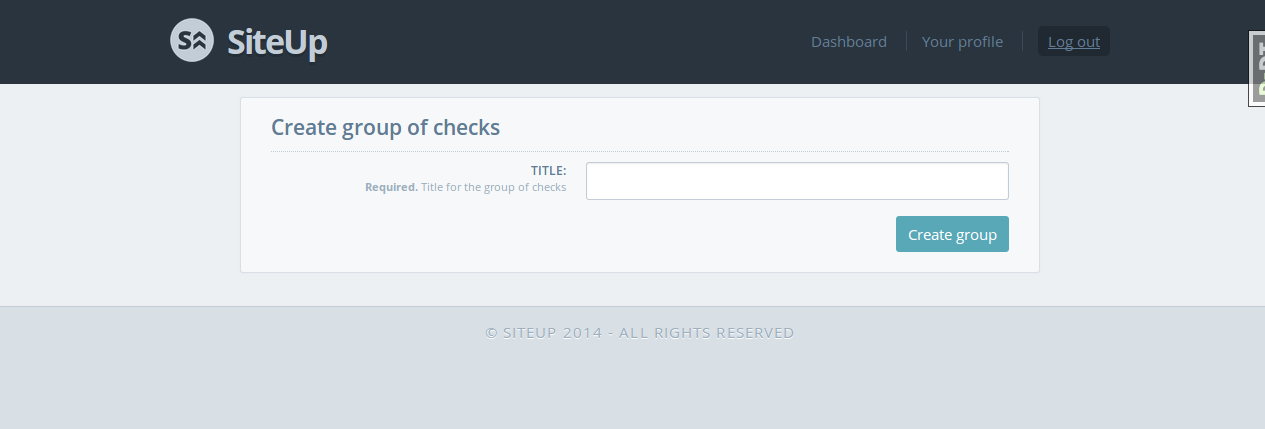
\includegraphics[width=\textwidth]{5_diseno/web-create-group}
  \caption{Pantalla de creación de grupo de chequeos}
  \label{fig:web-create-group}
\end{figure}

La figura~\ref{fig:web-create-group} representa la pantalla para crear un grupo
de chequeos. Muestra un formulario en el que hay que introducir los detalles del
grupo, concretamente el título que lo describe.

Cuando el usuario introduzca el título y pulse el botón, el sistema revisará que
los datos sean correctos. En caso afirmativo, el sistema creará el nuevo
grupo. En caso negativo, se volverá a mostrar el formulario, indicando los
fallos ocurridos.

% \vfill

\subsection{Pantallas de creación de chequeo}

\begin{figure}[htbp]
  \centering
  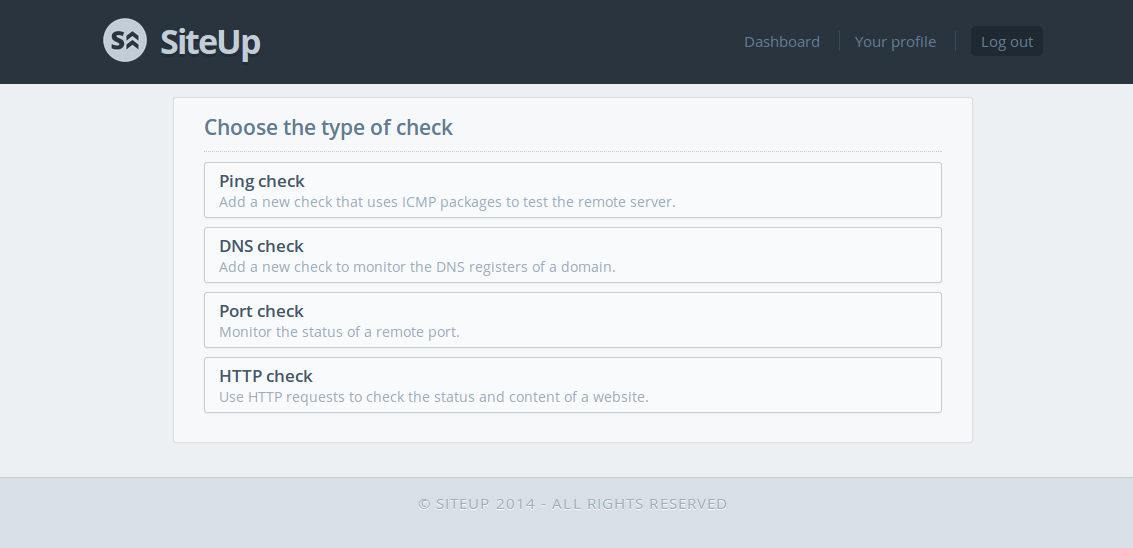
\includegraphics[width=\textwidth]{5_diseno/web-choose-type}
  \caption{Pantalla de elección de tipo de chequeo}
  \label{fig:web-choose-type}
\end{figure}

La creación de un chequeo se divide en dos pantallas principalmente. El primer
paso es elegir el tipo de chequeo a crear, mediante los botones que aparecen en
la pantalla de la figura~\ref{fig:web-choose-type}. 

Una vez elegido el tipo de chequeo a crear, aparecerá un formulario para
introducir los detalles del chequeo, que variará según el tipo de chequeo
elegido. En la figura~\ref{fig:web-create-check} se puede ver el formulario que
aparecerá a la hora de crear un chequeo de tipo DNS.

\begin{figure}[htbp]
  \centering
  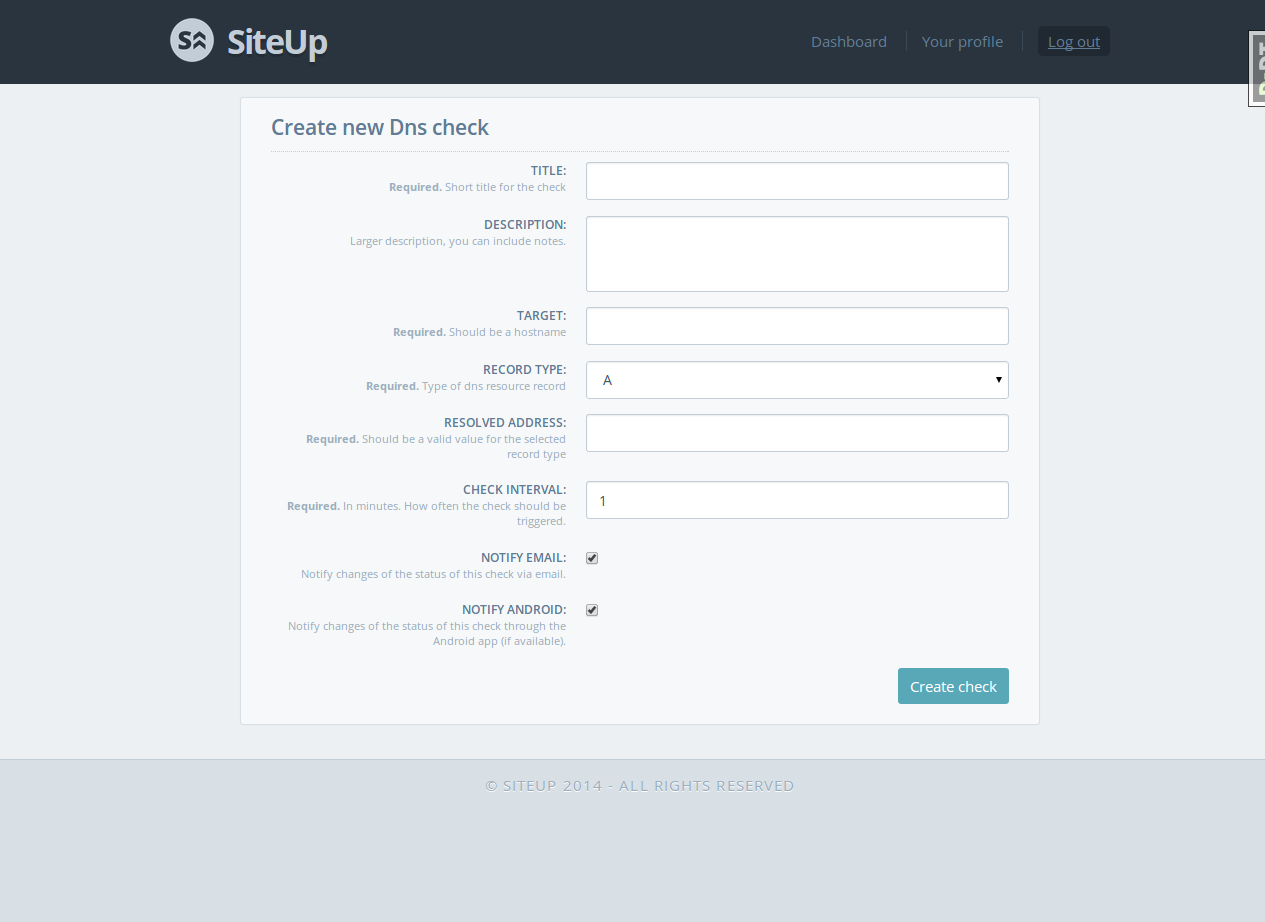
\includegraphics[width=\textwidth]{5_diseno/web-create-check}
  \caption{Pantalla de introducción de datos del chequeo}
  \label{fig:web-create-check}
\end{figure}


Cuando el usuario rellene el formulario y pulse el botón, se enviarán los datos
y el sistema comprobará que la información es correcta. En tal caso, se creará
el nuevo chequeo y se redirigirá al usuario al \textit{dashboard}. En caso
contrario, se volverá a mostrar el formulario, indicando los errores
encontrados.

\subsection{Pantalla genérica de borrado}

\begin{figure}[htbp]
  \centering
  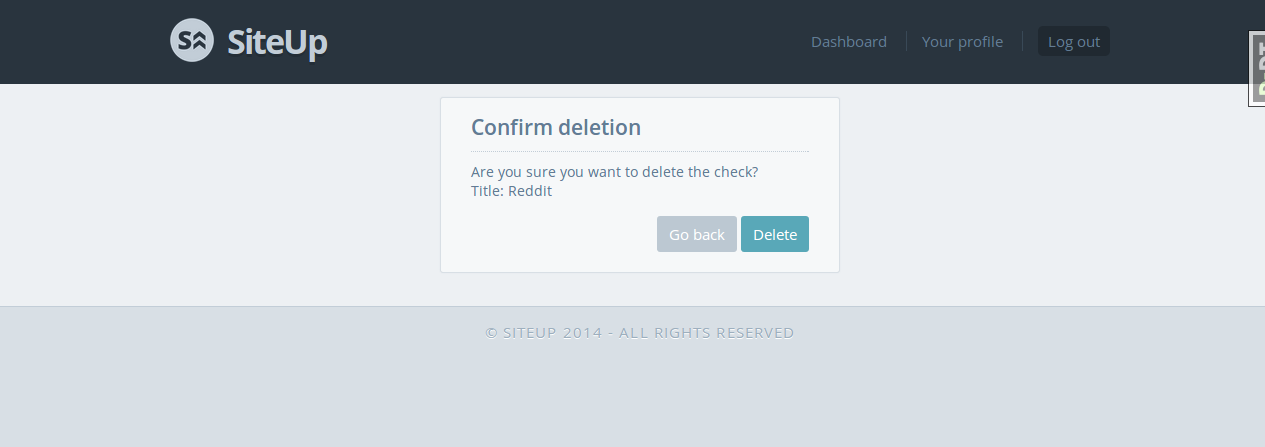
\includegraphics[width=\textwidth]{5_diseno/web-delete}
  \caption{Pantalla genérica de borrado}
  \label{fig:web-delete}
\end{figure}

En la figura~\ref{fig:web-delete} se representa la pantalla de confirmación de
borrado que aparece cuando se intenta borrar un chequeo o un grupo de
chequeos. La pantalla es sencilla: pregunta al usuario si desea realmente borrar
el elemento, ofreciendo dos botones, uno para confirmar el borrado y otro para
cancelar la operación. En ambos casos, tras la interacción el sistema redirige
al usuario al \textit{dashboard}.

\subsection{Pantalla del perfil de usuario}

\begin{figure}[htbp]
  \centering
  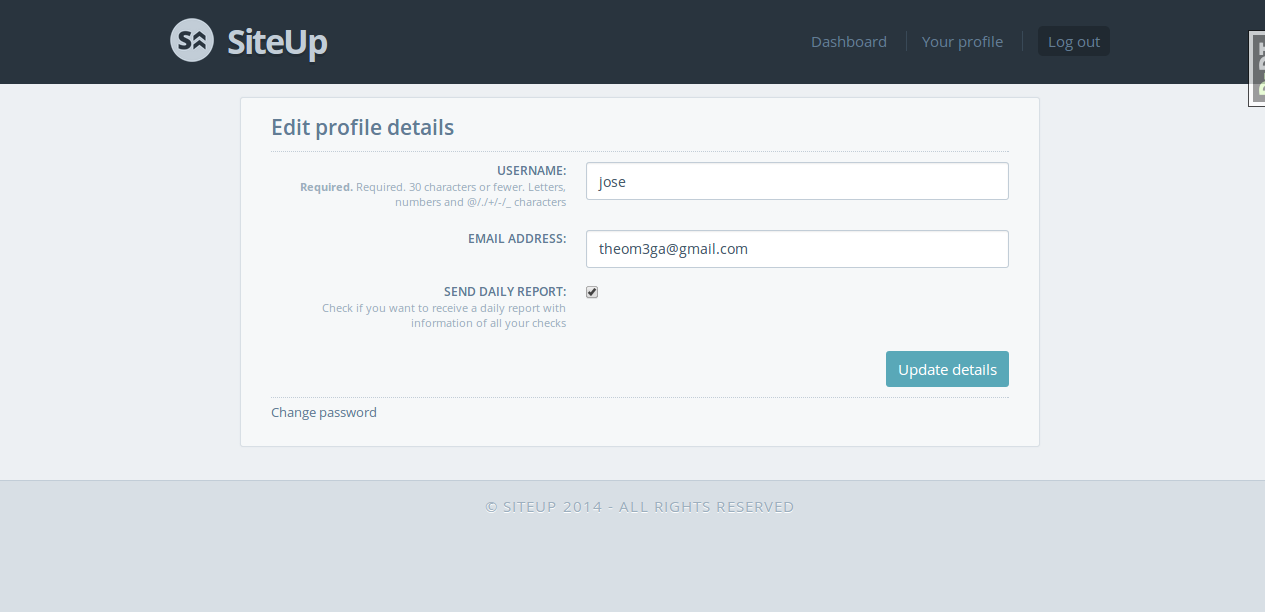
\includegraphics[width=\textwidth]{5_diseno/web-profile}
  \caption{Pantalla del perfil de usuario}
  \label{fig:web-profile}
\end{figure}

En la figura~\ref{fig:web-profile} se muestra la pantalla para editar el perfil
de usuario, a la que se llega pulsando el botón \textit{Your profile} situado en
la barra superior de navegación.

Desde esta pantalla el usuario puede modificar sus datos de usuario: nombre de
usuario, correo electrónico y si desea recibir un reporte diario sobre el estado
de sus chequeos.

También cuenta con la opción de cambiar la contraseña pulsando el botón
\textit{Change password}.


\FloatBarrier
\section{Diseño de la interfaz de usuario de la aplicación móvil}

En esta sección se detallarán las interfaces visuales de la aplicación móvil
para sistemas operativos Android, indicando la navegabilidad e interacción entre
las pantallas.


\subsection{Aspecto desde el lanzador}

\begin{figure}[htbp]
  \centering
  
\includegraphics[width=0.4\textwidth]{5_diseno/android-1}
  \caption{Icono de SiteUp en el lanzador}
  \label{fig:android-launcher}
\end{figure}

La figura~\ref{fig:android-launcher} muestra el aspecto del icono de la aplicación
desde el lanzador de aplicaciones de Android. 

Como se comentó en la sección~\ref{subsec:logotipo}, el logotipo fue diseñado
pensando en su legibilidad en bajas resoluciones, por lo que el icono de la
aplicación es fácilmente identificable desde el lanzador.

Al pulsar el icono de la aplicación, se lanza la pantalla de carga.

\subsection{Pantalla de carga}

\begin{figure}[htbp]
  \centering
  
\includegraphics[width=0.4\textwidth]{5_diseno/android-2}
  \caption{Pantalla de carga de la aplicación móvil}
  \label{fig:android-loading}
\end{figure}

En cuanto se pulsa el lanzador aparece la pantalla de carga de la aplicación,
visible en la figura~\ref{fig:android-loading}. Esta pantalla permanece visible
poco tiempo ya que el tiempo de carga es rápido.

Tras el proceso de carga, si la aplicación Android detecta que el usuario ha
iniciado sesión previamente, se carga la pantalla con el listado de chequeos. En
caso de que no haya datos de una sesión anterior, se carga la pantalla de login.

\subsection{Pantalla de inicio de sesión}

\begin{figure}[htbp]
  \centering
  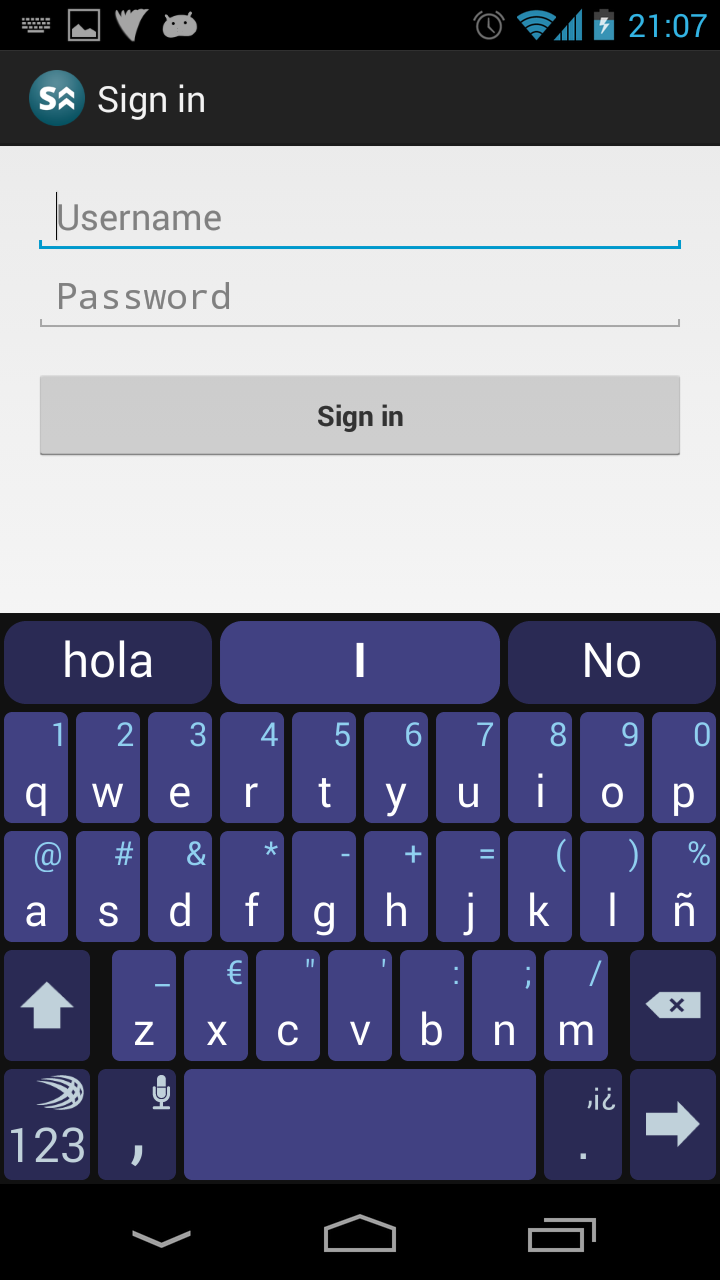
\includegraphics[width=0.4\textwidth]{5_diseno/android-3}
  \caption{Pantalla de inicio de sesión de la aplicación móvil}
  \label{fig:android-login}
\end{figure}

Tras cargar la aplicación, si no se detectan datos de inicio de sesión previos
se muestra la pantalla de inicio de sesión, visible en la
figura~\ref{fig:android-login}, en la que el usuario debe introducir su nombre
de usuario y contraseña para iniciar sesión.

\subsection{Pantalla de listado de chequeos}

\begin{figure}[p]
  \centering
  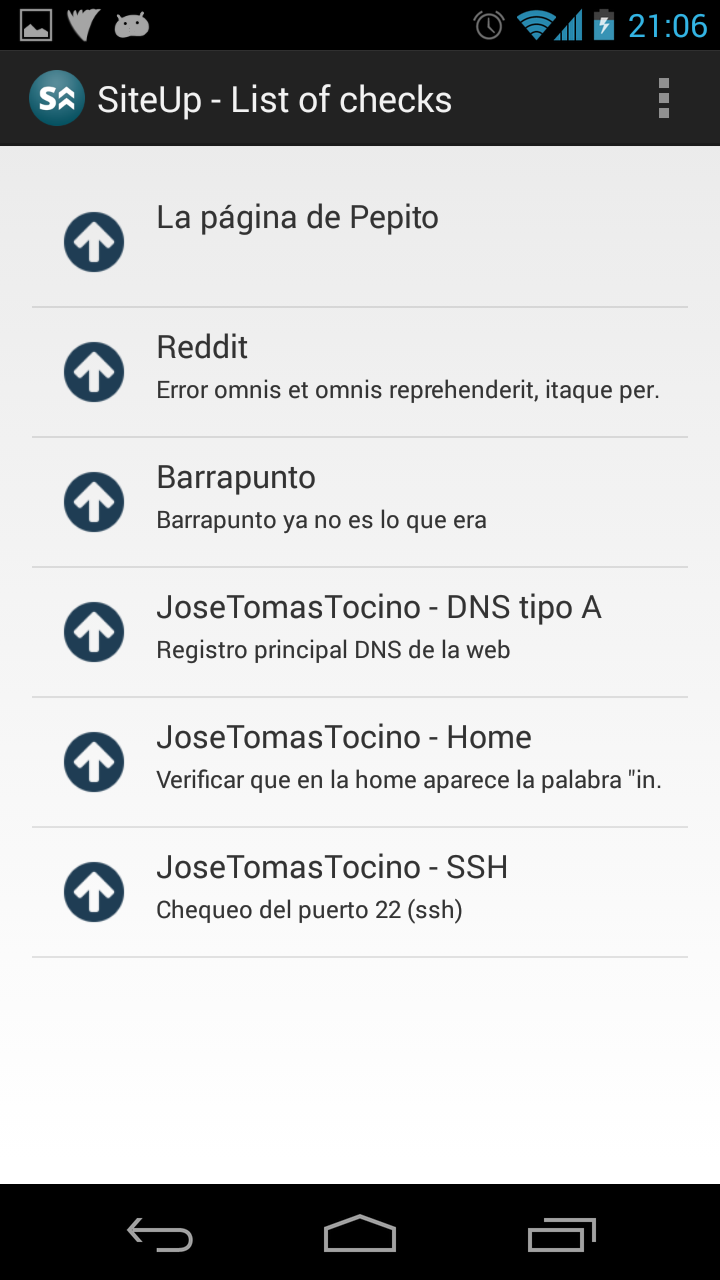
\includegraphics[width=0.4\textwidth]{5_diseno/android-4}
  \caption{Pantalla de chequeos de la aplicación móvil}
  \label{fig:android-dashboard}
\end{figure}

\begin{figure}[p]
  \centering
  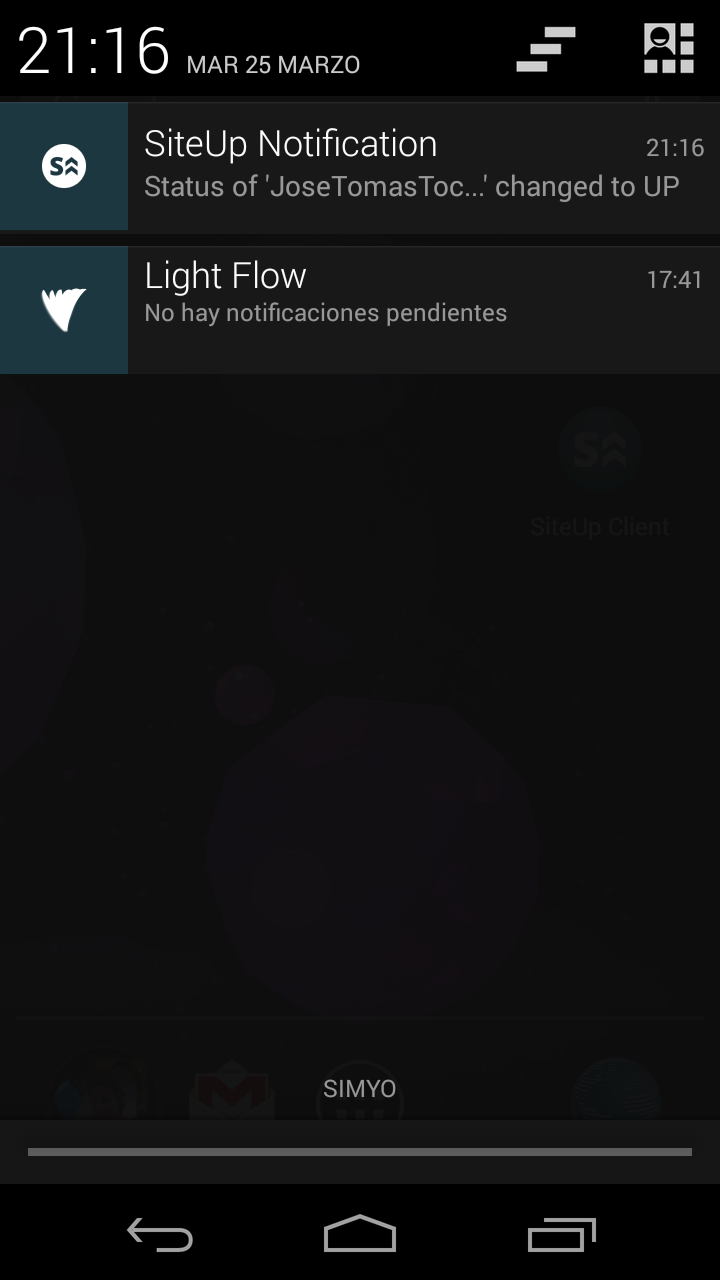
\includegraphics[width=0.4\textwidth]{5_diseno/android-5}
  \caption{Aspecto de las notificaciones}
  \label{fig:android-notification}
\end{figure}

La figura~\ref{fig:android-dashboard} muestra la pantalla con el listado de
chequeos del usuario. Desde aquí es posible cerrar la sesión de usuario, o
pulsar en alguno de los chequeos para ver sus detalles, lo cual abrirá un
navegador y mostrará la plataforma web.

\subsection{Notificación}



La figura~\ref{fig:android-notification} muestra el aspecto que tienen las
notificaciones que la aplicación es capaz de recibir. Desde estas notificaciones
es posible dirigirse a la web para ver los detalles del chequeo involucrado.

%%% Local Variables: 
%%% mode: latex
%%% TeX-master: "../memoria"
%%% End: 
